\documentclass[11pt,letter]{article}
\usepackage[top=1.00in, bottom=1.0in, left=1.1in, right=1.1in]{geometry}
\renewcommand{\baselinestretch}{1.1}
\usepackage{graphicx}
\usepackage{natbib}
\usepackage{amsmath}
\usepackage{textcomp}%amoung other things, it allows degrees C to be added
\usepackage{float}
\usepackage{hyperref}
\usepackage[utf8]{inputenc} % allow funny letters in citaions 
\usepackage{amsmath} % making nice equations 

\def\labelitemi{--}
\parindent=0pt

\title{Dashboard ideas for BC vin}
\date{\today}
\author{Faith Jones}

\graphicspath{ {./images/} }% tell latex where to find photos 

\begin{document}

\maketitle
\tableofcontents

\section{Background}

When we visited the winegrape growers in the Okenagan  Valley, Mike from Arterra mentioned that they are developing a dashboard for keeping track of the vineyard spraying schedules. This gave us the idea that maybe we could also have a dashboard for communicating with local growers. The dashboard could sit on our website, and be the main information source for the growers. 

If you are not sure what a dashboard is, I recommend taking a look at this one \url{https://coronavirus.jhu.edu/map.html}. What a dashboard does is show a map that on-line users can play with, along with some relevant plots and tables. The map should be using up to date data that is scraped from some on-line source.   

\section{What would we display?}
What I envision is a resource where growers can check information they need about the grape varieties they are growing. Initially I think we should focus on bud cold hardiness because we know that growers find this information very useful. At the moment Carl Bogdanoff from AgCanada emails growers periodically with predicted winegrape hardiness based on his model, but he is retiring this year. The growers find this information useful for planning when to take extra precautions to protect vines from freeze damage. \\

I do not know whether we should try and have a raster layer of predicted hardiness across the Okenagan valley, or predict values at a subset of points. Generally the dashboards I have seen have point data rather than raster data, maybe because it is handy to make plots and tables from it?\\

Eventually I think it would be cool to have phenology models on this or a similar dashboard as well. Maybe another dashboard that uses next year's predicted climate data to predict phenology? 

Here are some ideas for the type of visuals we could include:
\begin{itemize}
	\item A gouge or table showing minimum air temperature and maximum hardiness? Maybe split by variety?
	\item A line plot showing the air temperatures up to today and the predicted hardiness of the different varieties in the different locations. Users could chose what level of splitting the data they want, and what factors to show. For example, it would start with an average across all data, then the user could select an option to view varieties or locations separately. 
	\item A chart of some sort (barchart?) showing current hardiness of different varieties/locations. 
	\item We could have the option of colour-coding the points with hardiness values based on risk (i.e. blue when hardiness is much lower than air temp but increasing to red as air temperatures approach predicted hardiness).  
\end{itemize}
I made a quick sketch that might help visualise things, see Figure \ref{fig:DashboardSketchFJ}. 

\begin{figure}[H]
  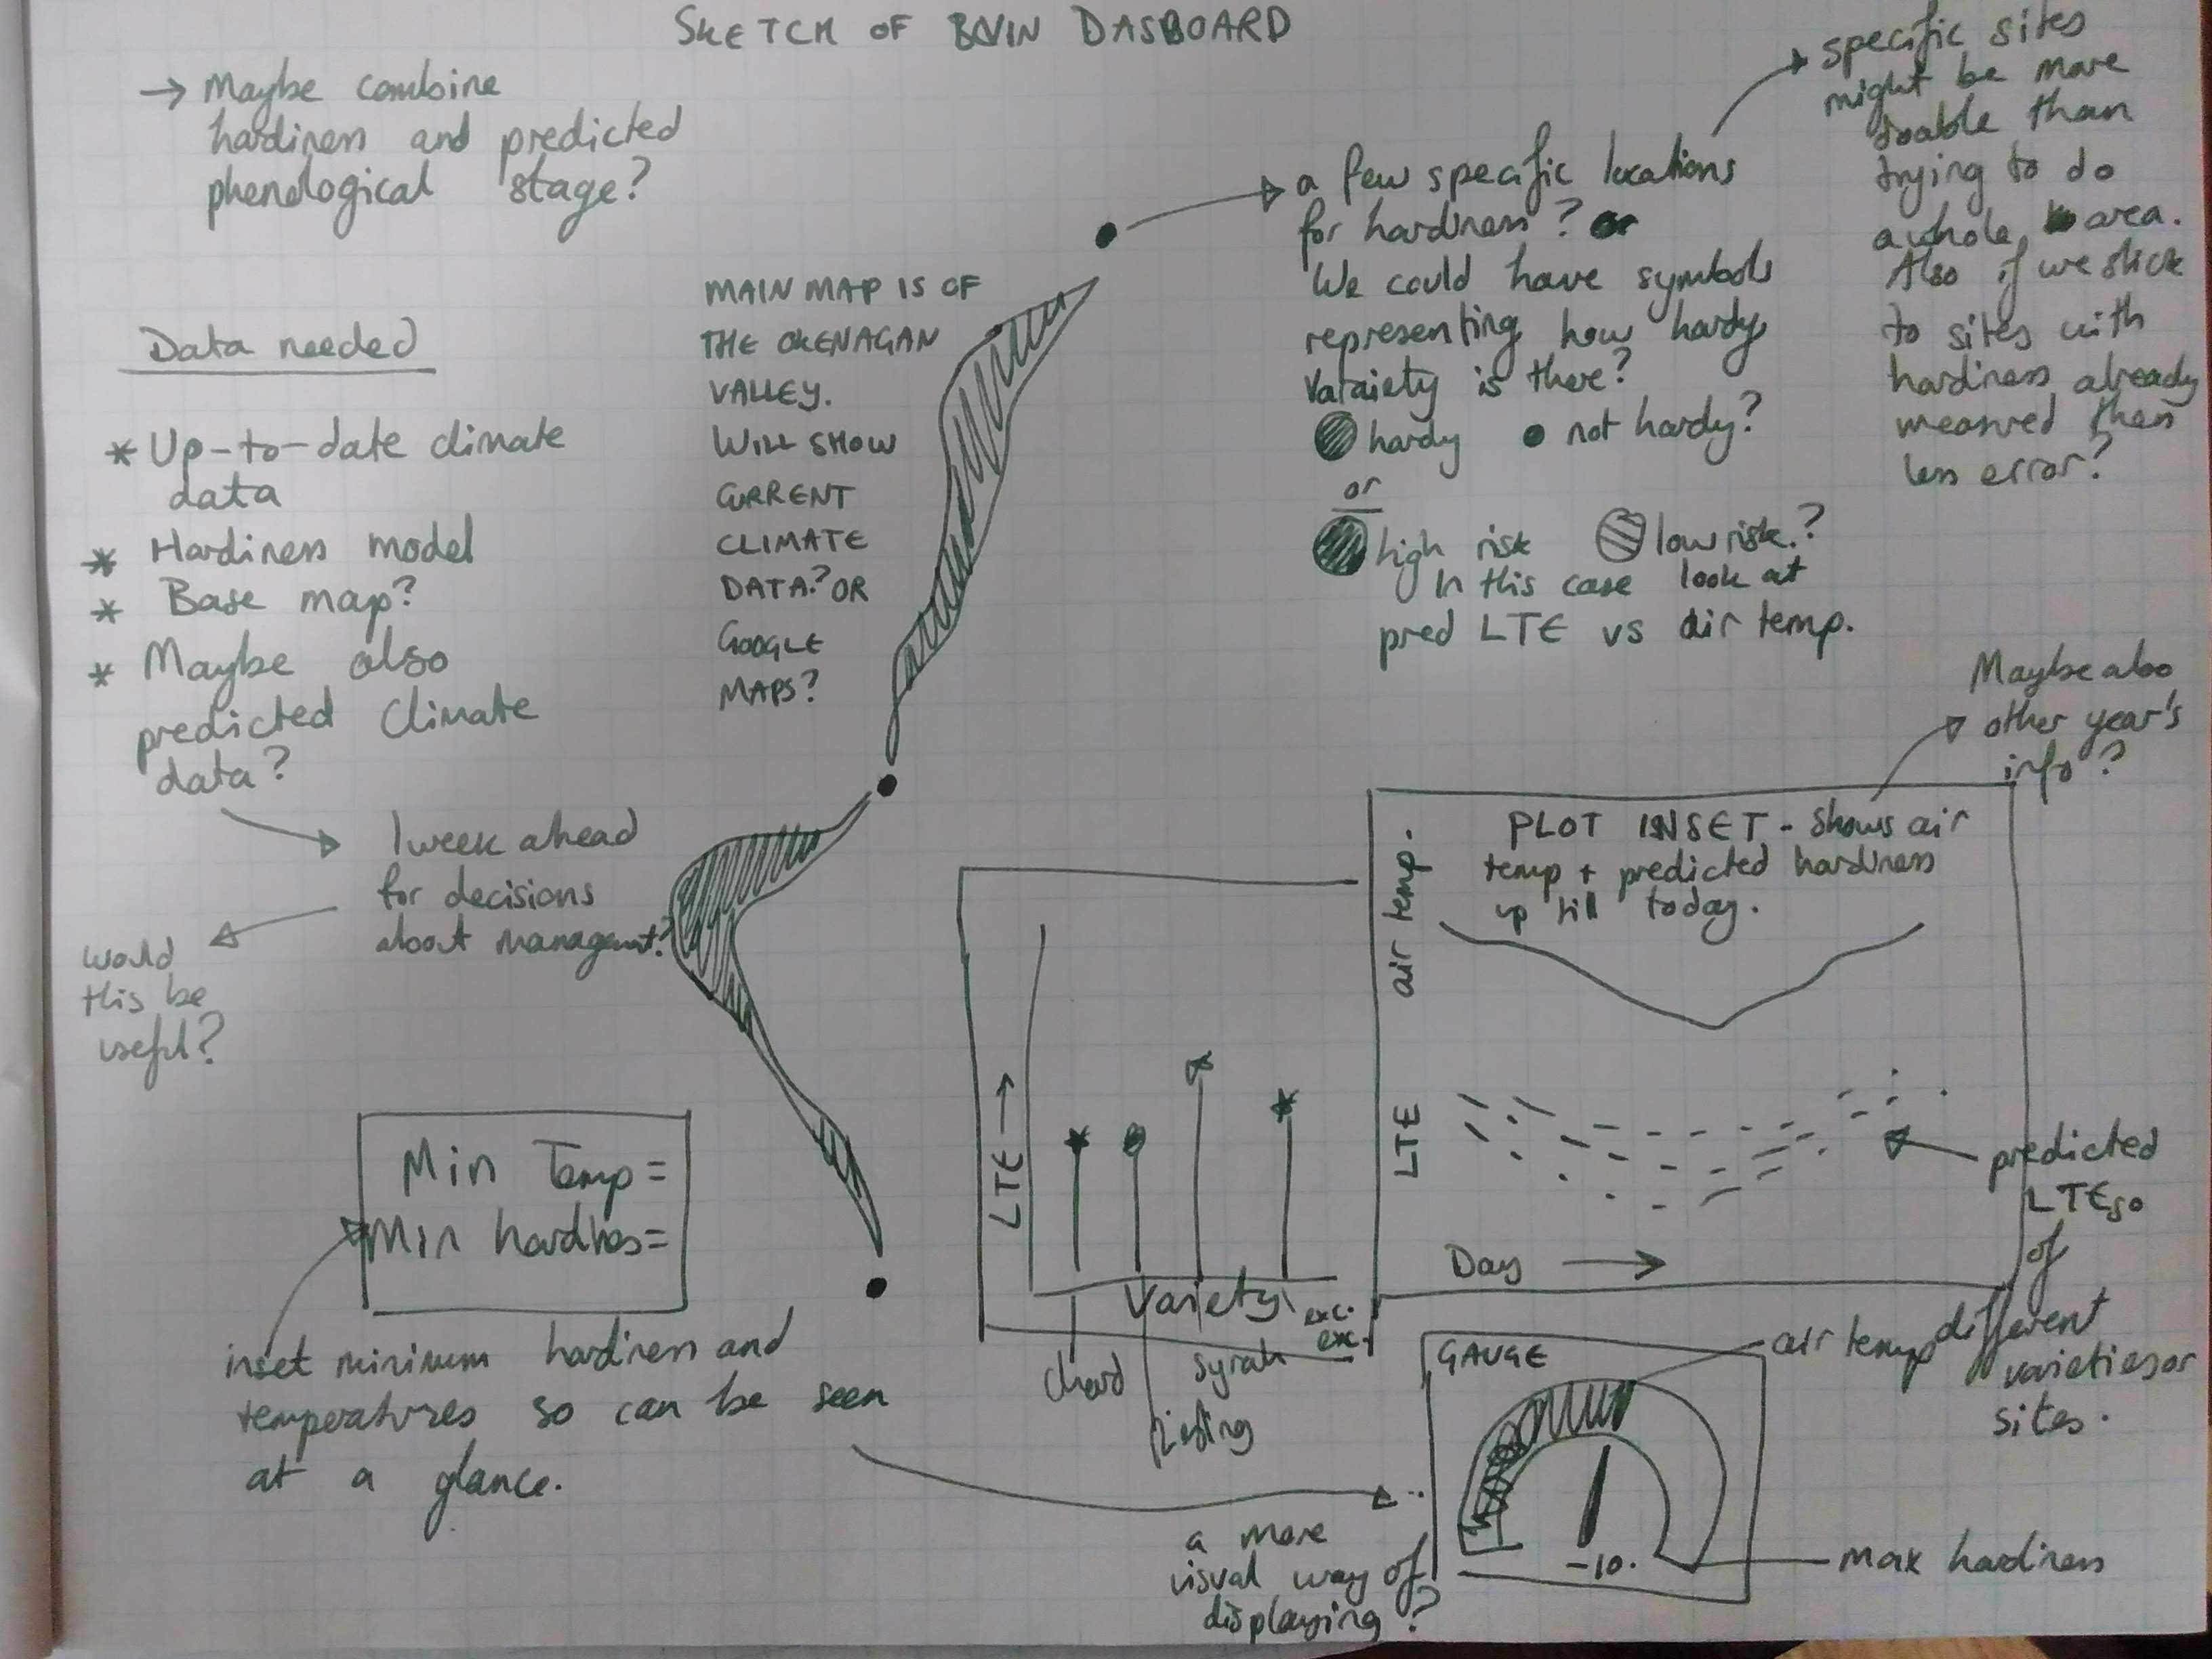
\includegraphics[width=\linewidth]{DashboardSketchFJ.jpg}
  \caption{A quick sketch Faith made on June 9th about what our cold hardiness dashboard could look like.}
  \label{fig:DashboardSketchFJ}
\end{figure}

\subsection{Data required}
\begin{itemize}
	\item Up to date climate data scraped from the Internet - what site?. 
	\item Maybe long term climate projections? Or might this be too complicated if the purpose is to inform growers on a week by week basis? Maybe projections are best provided as static maps?
	\item A hardiness model we can run the climate data through to get predicted bud cold hardiness values.  
	\item A base layer map - probably a simplified Google map?
	\item The location of the hardiness values. 
\end{itemize}

\section{How do we make a dashboard?}
I have never attempted something like this before, but here is what I have learned so far. To achieve a dashboard I think we need a we page to link it to. ALso we need some platform to build it. By far the most popular option is ESRI's ArgGIS Online tool (\url{https://www.esri.com/en-us/arcgis/products/arcgis-dashboards/overview}). These are slick and professional looking, and there are a lot of tutorials on-line to help. Unfortunately there is also a subscription fee. I have contacted our IT people because it is possible that UBC Forestry already has a subscription we could tap into. QGIS, an open source and free mapping program, might provide an alternative, but I do not think it is as slick and I think it is just a map rather than map and graphs (see \url{https://www.qgistutorials.com/en/docs/web_mapping_with_qgis2web.html}  and \url{https://qgiscloud.com/}). Another alternative might be to use R. This page \url{https://shiny.rstudio.com/articles/dashboards.html} suggests either the flexdashboard or the shinydashboard packages. See \url{https://rstudio.github.io/shinydashboard/structure.html} for how to use Shiny. I just looked briefly but it looks like it would do the job. Lizzie strongly prefers the R rout, and over the summer Adam Fong made some progress in this respect. I am not exactly sure what he did because I haven't got the code working on my computer yet, but the code is in bcvin\/hardiness\/dashboard. Adam also got a hardiness model designed by Carl from AgCanada working in R, but again I am getting error messages when I run the code. Once we have the model and dashboard code up and running we should have a better idea of where we are at.           

\section{Next steps}

We need to:
\begin{itemize}
	\item Decide what we want the dashboard to do and how it should look
	\item Get Adam's code to work and see what he has achieved 
	\item Figure out how to scrape data and where to get data from
	\item Chose a hardiness model - probably the one Adam has coded up that we got from Carl
	\item Figure out how to make a dashboard!
	\item Decide who should host the dashboard 
\end{itemize}
\end{document}


 
